\section{Zabezpečení dat}
Pokud detekujeme optickým přijímačem data, nikdy nemáme jistotu, že to jsou opravdu ta data která vyslal náš vysílač a nebo jestli jsou poškozena. K tomu abychom odhalili chybu v datech slouží zabezpečovací metody přenosu dat. Fungují na tom princcipu, že kromě dat samotných se posílá ještě další redundantní informace spočítaná s přenášených dat. Nekteré zabezpečovací algoritmy jsou schopny kromě detekce chyb i chyby opravovat, ale těmi se v této práci zabývat nebudu.

\subsection{Parita}
Parita je jednoduchý způsob zabezpečení dat. Ke každému slovu přenášených dat přidá jeden redundantní bit označovaný jako paritní. Rozližujeme ji na sudou a lichou.

\subsubsection{Sudá parita}
Paritní bit je nastaven tak, aby celkový počet jedniček v datovém slově včetně bitu paritního byl sudý. Můžeme ho spočítat jako exkluzivní součet všechy bitů datového slova.
$$ P_{sudá} = b_0 \oplus b_1 \oplus ... \oplus b_n $$

\begin{figure}[H]
    \begin{center}
        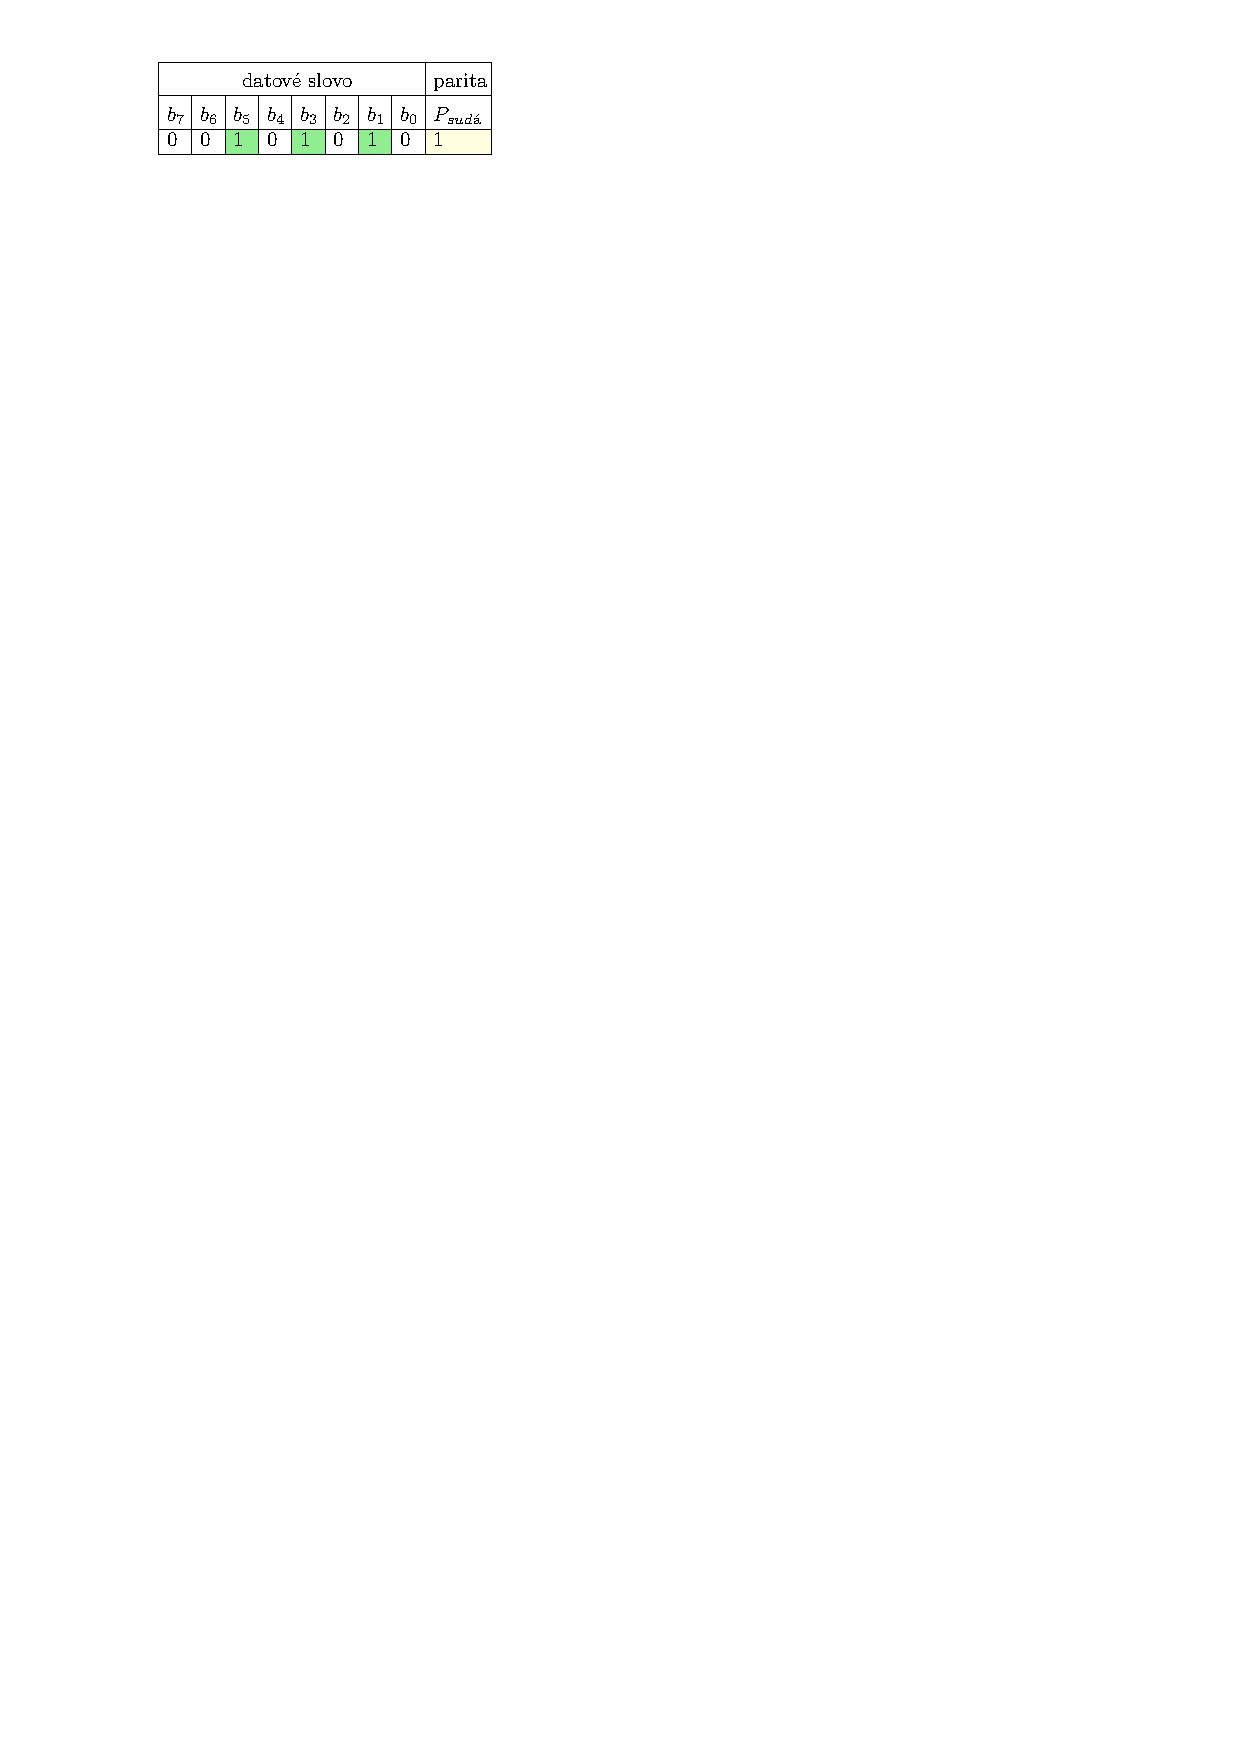
\includegraphics[scale=1]{img/parita_suda}
    \end{center}
    \caption{Ukázka sudé parity}
\end{figure}

\subsubsection{Lichá parita}
Paritní bit je nastaven tak, aby celkový počet jedniček v datovém slově včetně bitu paritního byl lichý. Můžeme ho spočítat obdobně jako sudý paritní bit, jen výsledek musíme znegovat.
$$ P_{lichá} = \overline{ b_0 \oplus b_1 \oplus ... \oplus b_n } $$

\begin{figure}[H]
    \begin{center}
        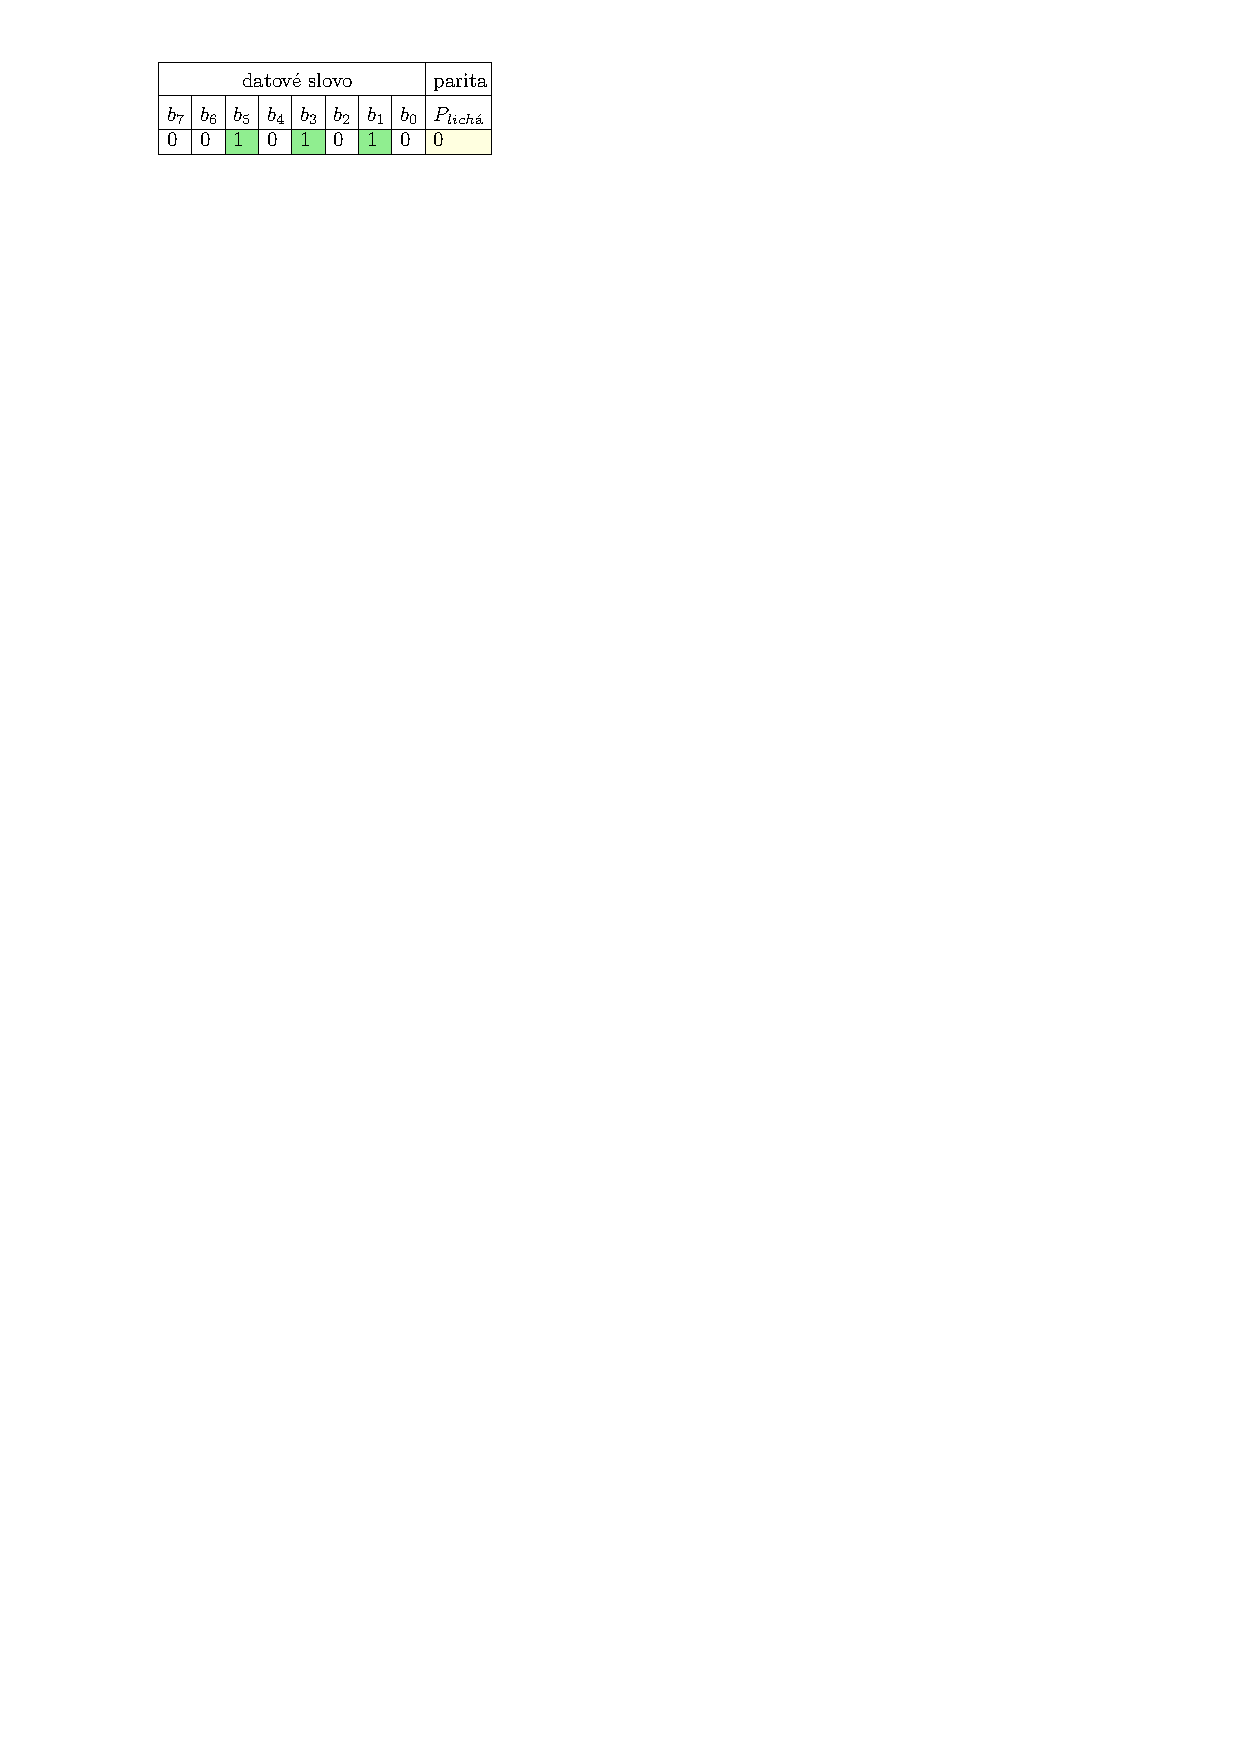
\includegraphics[scale=1]{img/parita_licha}
    \end{center}
    \caption{Ukázka liché parity}
\end{figure}

\subsection{Cyklický redundantní součet}
